\section{Rational Zero Theorem}\label{subsec:s_polynomials}

\subsection{Statement}

The rational zero theorem states that each rational zero(s) of a polynomial with integer coefficients 
\begin{equation}
f(x) = a_nx^n+a_{n-1}x^{n-1}+.......+a_2x^2+a_1x+a_0
\end{equation}
is of the form $\frac{p}{q}$, where
\begin{itemize}
\item $p$ is a factor of the constant $a_0$ (the one without the $x$)
\item $q$ is a factor of the leading coefficient $a_n$ (the one with the highest power of $x$)
\item $p$ and $q$ are relatively prime (i.e., the fraction $\frac{p}{q}$ is in its simplest form)

Example: 6 and 18 are not relatively prime because the fraction $\frac{6}{18}$ can be simplified to $\frac{1}{3}$
\item The integer coefficients are positive or negative integers: $a_{i}\in \mathbb{Z}$ 

This means that the theorem cannot be applied to a polynomial like $\frac{1}{3}x^3+\sqrt{2}x+3$.
\item $a_{0}$ , $a_{n}\neq 0$.
\end{itemize}

In other words

\begin{equation}
\frac{p}{q} = \frac{\textrm{factor of }a_0}{\textrm{factor of }a_n}
\end{equation}

Example:

\begin{equation}
2x^3-5x^2-4x+3=0
\end{equation}

\begin{itemize}
\item $p=\textrm{all the prime factors of 3, positive or negative:} \pm 1 \pm 3$
\item $q=\pm 1\pm 2$
\end{itemize}

\subsection{Usage}


We can use the Rational Zeros Theorem to find all the rational zeros of a polynomial. Here are the steps:
\begin{enumerate}
\item Arrange the polynomial in descending order\

(In the example: $2$, $-5$, $-4$, $3$)
\item Write down all the factors of the constant term.

These are all the possible values of $p$. ($p=\pm 1 \pm 3$)
\item Write down all the factors of the leading coefficient. 

These are all the possible values of $q$. ($q=\pm 1\pm 2$)
\item Write down all the possible values of $\pm \frac{p}{q}$.

Simplify each value and cross out any duplicates.  ( $\pm 1 \pm \frac{1}{2} \pm 3 \pm \frac{3}{2}$ )
\item Use the division algorithm to determine the values of for which $P(x) = 0$.

These are all the rational roots of $P(x)$.
\end{enumerate}


\section{Long division with polynomials}

\setcounter{equation}{0}
È un algoritmo per calcolare la divisione tra un polinomio e un altro.

% https://www.youtube.com/watch?v=_FSXJmESFmQ
\subsection{Esempio uno}

Dividere $x^2+5x+6$ (il dividendo) per $x+2$ (il divisore).

Si incomincia a scrivere così:

\begin{figure}[H]
\centering
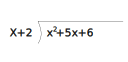
\includegraphics[width=0.8\textwidth]{polynomials.1.1.pdf}
\end{figure}

Si divide il termine più elevato del dividendo per il termine più elevato del divisore, in questo caso si divide $x^2$ per $x$.

$\frac{x^2}{x}=x$: il risultato è x, e si scrive in cima:

\begin{figure}[H]
\centering
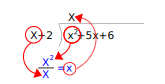
\includegraphics[width=0.8\textwidth]{polynomials.1.2.pdf}
\end{figure}

Ora moltiplico questo risultato ($x$) per il divisore ($x-2$):

\begin{equation}
(x+2)x=x^2+2x = x^2+x+0
\end{equation}

Notare che ho aggiunto $+0$ alla fine.

Ora faccio una sottrazione tra il dividendo ( $x^2+5x+6$ )e il risultato che ho trovato ora ($x^2+2x+0$).

Il risultato ($3x+6$) va scritto aggiungendo una riga in basso.

\begin{figure}[H]
\centering
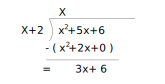
\includegraphics[width=0.8\textwidth]{polynomials.1.4.pdf}
\end{figure}

\begin{minipage}{\textwidth}
Adesso faccio la stessa cosa di prima: prendo il termine con il grado più alto del $3x+6$ e cioè $3x$, e lo divido per il termine con il grado più alto del divisore ($x-2$), che è $x$.

Il risultato della divisione ($3$) va in cima, di seguito al risultato del passaggio precedente.

\begin{figure}[H]
\centering
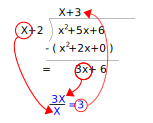
\includegraphics[width=0.8\textwidth]{polynomials.1.5.pdf}
\end{figure}
\end{minipage}

Esattamente come prima, moltiplico questo $3$ che ho trovato adesso per il divisore ($x-2$):

\begin{equation}
(x+2)3=3x+6
\end{equation}

Il risultato trovato ($3x+6$) va sottratto all'ultima riga del passaggio precedente:


\begin{figure}[H]
\centering
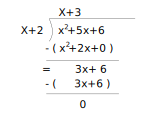
\includegraphics[width=0.8\textwidth]{polynomials.1.7.pdf}
\end{figure}

Il risultato è zero, quindi non c'è resto.

La soluzione del problema iniziale è:

\begin{equation}
\frac{x^2+5x+6}
{x+2} = x+3
\end{equation}

\begin{minipage}{\textwidth}
\subsection{Esempio due}

\setcounter{equation}{0}

\begin{equation}
\frac{2x^3+8x^2-6x+10}{x-2}
\end{equation}


\begin{figure}[H]
\centering
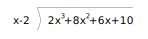
\includegraphics[width=0.8\textwidth]{polynomials.2.1.pdf}
\end{figure}

Prendo il termine di grado maggiore del dividendo ($2x^3$) e lo divido per il termine di grado maggiore del divisore ($x$).

\begin{equation}
\frac{2x^3}
{x} = 2x^2
\end{equation}

Questo $2x^2$ lo scrivo in cima come primo termine del risultato finale.

Faccio la moltiplicazione di questo primo termine ($2x^2$) per il divisore ($x-2$):

\begin{equation}
(x-2)2x^2 = 2x^3-4x^2
\end{equation}

e lo scrivo in basso aggiungendo una riga, per fare la sottrazione:

\begin{figure}[H]
\centering
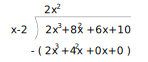
\includegraphics[width=0.8\textwidth]{polynomials.2.2.pdf}
\end{figure}

\end{minipage}

La sottrazione è questa:

\begin{equation}
2x^3+8x^2-6x+10 - (  2x^3+4x^2+0x+0 )= 12x^2-6x+10
\end{equation}

Il risultato lo scrivo sotto aggiungendo una riga.

\begin{figure}[H]
\centering
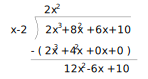
\includegraphics[width=0.8\textwidth]{polynomials.2.3.pdf}
\end{figure}

Adesso prendo il termine di grado maggiore che sta nell'ultima riga appena scritta ($12x^2$) e lo divido per il termine di grado maggiore del divisore ($x$).

\begin{equation}
\frac{12x^2}
{x} = 12x
\end{equation}

Questo $12x$ viene scritto come secondo termine del risultato finale.


\begin{figure}[H]
\centering
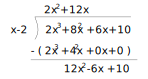
\includegraphics[width=0.8\textwidth]{polynomials.2.4.pdf}
\end{figure}

Adesso tocca alla moltiplicazione:

\begin{equation}
12x * (x-2) = 12x^2-24x
\end{equation}

Lo scrivo sotto aggiungendo una riga e faccio la sottrazione:

\begin{equation}
12x^2-6x+10-( 12x^2-24x ) = 18x+10
\end{equation}

\begin{figure}[H]
\centering
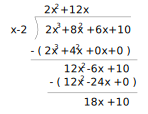
\includegraphics[width=0.8\textwidth]{polynomials.2.5.pdf}
\end{figure}

Il risultato è $18x+10$.

Il prossimo passo è la divisione 

\begin{equation}
\frac{18x}{x}=18
\end{equation}

Scrivo questo 18 come terzo termine del risultato finale, e faccio la moltiplicazione
\begin{equation}
18*(x-2) = 18x-36
\end{equation}

Aggiungo $18x-36$ come ultima riga e faccio la sottrazione.

\begin{figure}[H]
\centering
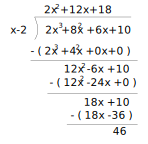
\includegraphics[width=0.8\textwidth]{polynomials.2.6.pdf}
\end{figure}

Il risultato da scrivere in fondo è 46.

Non si può più andare avanti; $\frac{46}{x-2}$ resta così, e il risultato finale dell'operazione è questo:

\begin{equation}
\frac{2x^3+8x^2-6x+10}{x-2} = 2x^2+12x+18+\frac{46}{x-2}
\end{equation}

\subsection{Esercizi}

\begin{enumerate}
\item A polynomial $P(x)=2x^3-5x^2-4x+3$ is given.
\begin{enumerate}
\item List all possible rational zeros of P
\item Find all real zeros of P
\item Sketch the graph of P
\end{enumerate}

\rightline{( Soluzione a pagina \pageref{poli_1} \label{exp_1}\label{exp_1} )}

\end{enumerate}
